
\documentclass[a4paper,11pt]{article}
\usepackage[a4paper, margin=8em]{geometry}

% usa i pacchetti per la scrittura in italiano
\usepackage[french,italian]{babel}
\usepackage[T1]{fontenc}
\usepackage[utf8]{inputenc}
\frenchspacing 

% usa i pacchetti per la formattazione matematica
\usepackage{amsmath, amssymb, amsthm, amsfonts}

% usa altri pacchetti
\usepackage{gensymb}
\usepackage{hyperref}
\usepackage{standalone}

% imposta il titolo
\title{Appunti Fondamenti di Automatica}
\author{Luca Seggiani}
\date{2025}

% disegni
\usepackage{pgfplots}
\pgfplotsset{width=10cm,compat=1.9}

% imposta lo stile
% usa helvetica
\usepackage[scaled]{helvet}
% usa palatino
\usepackage{palatino}
% usa un font monospazio guardabile
\usepackage{lmodern}

% tikz in sans
\tikzset{every picture/.style={/utils/exec={\sffamily}}}

\renewcommand{\rmdefault}{ppl}
\renewcommand{\sfdefault}{phv}
\renewcommand{\ttdefault}{lmtt}

% circuiti
\usepackage{circuitikz}
\usetikzlibrary{babel}

% disponi il titolo
\makeatletter
\renewcommand{\maketitle} {
	\begin{center} 
		\begin{minipage}[t]{.8\textwidth}
			\textsf{\huge\bfseries \@title} 
		\end{minipage}%
		\begin{minipage}[t]{.2\textwidth}
			\raggedleft \vspace{-1.65em}
			\textsf{\small \@author} \vfill
			\textsf{\small \@date}
		\end{minipage}
		\par
	\end{center}

	\thispagestyle{empty}
	\pagestyle{fancy}
}
\makeatother

% disponi teoremi
\usepackage{tcolorbox}
\newtcolorbox[auto counter, number within=section]{theorem}[2][]{%
	colback=blue!10, 
	colframe=blue!40!black, 
	sharp corners=northwest,
	fonttitle=\sffamily\bfseries, 
	title=Teorema~\thetcbcounter: #2, 
	#1
}

% disponi definizioni
\newtcolorbox[auto counter, number within=section]{definition}[2][]{%
	colback=red!10,
	colframe=red!40!black,
	sharp corners=northwest,
	fonttitle=\sffamily\bfseries,
	title=Definizione~\thetcbcounter: #2,
	#1
}

% disponi problemi
\newtcolorbox[auto counter, number within=section]{problem}[2][]{%
	colback=green!10,
	colframe=green!40!black,
	sharp corners=northwest,
	fonttitle=\sffamily\bfseries,
	title=Problema~\thetcbcounter: #2,
	#1
}

% disponi codice
\usepackage{listings}
\usepackage[table]{xcolor}

\lstdefinestyle{codestyle}{
		backgroundcolor=\color{black!5}, 
		commentstyle=\color{codegreen},
		keywordstyle=\bfseries\color{magenta},
		numberstyle=\sffamily\tiny\color{black!60},
		stringstyle=\color{green!50!black},
		basicstyle=\ttfamily\footnotesize,
		breakatwhitespace=false,         
		breaklines=true,                 
		captionpos=b,                    
		keepspaces=true,                 
		numbers=left,                    
		numbersep=5pt,                  
		showspaces=false,                
		showstringspaces=false,
		showtabs=false,                  
		tabsize=2
}

\lstdefinestyle{shellstyle}{
		backgroundcolor=\color{black!5}, 
		basicstyle=\ttfamily\footnotesize\color{black}, 
		commentstyle=\color{black}, 
		keywordstyle=\color{black},
		numberstyle=\color{black!5},
		stringstyle=\color{black}, 
		showspaces=false,
		showstringspaces=false, 
		showtabs=false, 
		tabsize=2, 
		numbers=none, 
		breaklines=true
}

\lstdefinelanguage{javascript}{
	keywords={typeof, new, true, false, catch, function, return, null, catch, switch, var, if, in, while, do, else, case, break},
	keywordstyle=\color{blue}\bfseries,
	ndkeywords={class, export, boolean, throw, implements, import, this},
	ndkeywordstyle=\color{darkgray}\bfseries,
	identifierstyle=\color{black},
	sensitive=false,
	comment=[l]{//},
	morecomment=[s]{/*}{*/},
	commentstyle=\color{purple}\ttfamily,
	stringstyle=\color{red}\ttfamily,
	morestring=[b]',
	morestring=[b]"
}

% disponi sezioni
\usepackage{titlesec}

\titleformat{\section}
	{\sffamily\Large\bfseries} 
	{\thesection}{1em}{} 
\titleformat{\subsection}
	{\sffamily\large\bfseries}   
	{\thesubsection}{1em}{} 
\titleformat{\subsubsection}
	{\sffamily\normalsize\bfseries} 
	{\thesubsubsection}{1em}{}

% disponi alberi
\usepackage{forest}

\forestset{
	rectstyle/.style={
		for tree={rectangle,draw,font=\large\sffamily}
	},
	roundstyle/.style={
		for tree={circle,draw,font=\large}
	}
}

% disponi algoritmi
\usepackage{algorithm}
\usepackage{algorithmic}
\makeatletter
\renewcommand{\ALG@name}{Algoritmo}
\makeatother

% disponi numeri di pagina
\usepackage{fancyhdr}
\fancyhf{} 
\fancyfoot[L]{\sffamily{\thepage}}

\makeatletter
\fancyhead[L]{\raisebox{1ex}[0pt][0pt]{\sffamily{\@title \ \@date}}} 
\fancyhead[R]{\raisebox{1ex}[0pt][0pt]{\sffamily{\@author}}}
\makeatother

\begin{document}

% sezione (data)
\section{Lezione del 02-04-25}

% stili pagina
\thispagestyle{empty}
\pagestyle{fancy}

% testo
\subsubsection{Esempio: conversione dalla forma a stato alla funzione di trasferimento}
Prendiamo l'esempio di una forma a variabili di stato arbitraria e riportiamola in funzione di trasferimento:
\[
	\begin{cases}
		x' = 
		\begin{pmatrix}
			0 & 1 & 0 \\ 0 & 0 & 1 \\ -1 & -2 & -3
		\end{pmatrix}
		x +
		\begin{pmatrix}
			10 \\ 0 \\ 0
		\end{pmatrix}
		u \\ 
		y =
		\begin{pmatrix}
			1 & 0 & 0
		\end{pmatrix}
		x
	\end{cases}
\]
Dalla matrice $A$ ricaviamo $sI - A$:
$$
sI - A =
\begin{pmatrix}
	s & -1 & 0 \\
	0 & s & -1 \\ 
	1 & 2 & s + 3
\end{pmatrix}
$$
da cui l'inversa:
$$
(sI - A)^{-1} =
\frac{1}{s^3 + 3s^2 + 2s + 1}
\begin{pmatrix}
	s^2 + 3s - 2 & s + 3 & 1 \\ 
	-1 & s^2 + 3s & s \\ 
	-s & -2s - 1 & s^2
\end{pmatrix}
$$
dove notiamo come sempre il denominatore è il polinomio dato da $a_n ... a_1$.
Applichiamo quindi la formula completa:
$$
G(s) = C (sI - A)^{-1} B \, ( + D ) = 
\begin{pmatrix}
	1 & 0 & 0
\end{pmatrix}
\frac{1}{s^3 + 3s^2 + 2s + 1}
\begin{pmatrix}
	s^2 + 3s - 2 & s + 3 & 1 \\ 
	-1 & s^2 + 3s & s \\ 
	-s & -2s - 1 & s^2
\end{pmatrix}
\begin{pmatrix}
	10 \\ 0 \\ 0
\end{pmatrix}
$$
$$
\begin{pmatrix}
	1 & 0 & 0
\end{pmatrix}
\frac{1}{s^3 + 3s^2 + 2s + 1}
\begin{pmatrix}
	10s^2 + 30s - 20 \\ 
	-10 \\
	-10s
\end{pmatrix}
= \frac{10s^2 + 30s - 20}{s^3 + 3s^2 + 2s + 1}
$$

\subsubsection{Matrici di trasferimento dei sistemi MIMO}
Abbiamo visto finora la funzione di trasferimento come una funzione scalare della variabile $s$.
Abbiamo in verità che questa può essere rappresentata in sistemi MIMO come:
$$
\mathbf{G}(s) = C (sI - A)^{-1} B =
\begin{pmatrix}
	g_{11}(s) & ... & g_{1m}(s) \\
	\vdots & \ddots & \vdots \\ 
	g_{p1}(s) & ... & g_{pm}(s) \\
\end{pmatrix}
$$
cioè una matrice che lega il trasferimento da ogni canale di ingresso a ogni canale di uscita, con $g_{ij}(s)$ funzione di trasferimento dal canale $u_j$ all'uscita $y_i$.

\subsubsection{Esempio: funzione di trasferimento della velocità di crociera}
Riprendiamo un'ennesima volta l'esempio 3.0.1, ricavandone la forma in funzione di trasferimento.
Avevamo che questo era rappresentato dal sistema:
\[
	\begin{cases}
		x' = \begin{pmatrix}
			0 & 1 \\ 0 & -\frac{\beta}{m}
		\end{pmatrix}	
		x + \begin{pmatrix}
			0 & 0 \\ \frac{\gamma}{m} & - g
		\end{pmatrix}
		u \\
		y = \begin{pmatrix}
			0 & 1
		\end{pmatrix}
		x
	\end{cases}
\]
da cui:
$$
sI - A = \begin{pmatrix}
	s & -1 \\
	0 & s + \frac{\beta}{m}
\end{pmatrix}, \quad
(sI - A)^{-1} =
\frac{1}{s\left( s + \frac{\beta}{m} \right)}
\begin{pmatrix}
	s + \frac{\beta}{m} & 1 \\
	0 & s
\end{pmatrix}
$$
Applicando la formula:
$$
\mathbf{G}(s) = C(sI - A)^{-1} B = \frac{1}{s\left(s + \frac{\beta}{m}\right)}
\begin{pmatrix}
	s \frac{\gamma}{m} - sg
\end{pmatrix}
= \begin{pmatrix}
	\frac{\gamma}{m \left( s + \frac{\beta}{m} \right)} &
	\frac{-g}{s + \frac{\beta}{m}}
\end{pmatrix}
$$

Avremo quindi una funzione di trasferimento $2\times 1$, dove le due entrate rappresentano rispettivamente l'effetto della propulsione del motore (che era $\gamma u$) e dell'accelerazione gravitazionale.
Visto che sulla seconda non si può agire, prenderemo in interesse la prima entrata:
$$
G(s) = \frac{\gamma}{m \left( s + \frac{\beta}{m} \right)}
$$

Di questa potremmo ad esempio prendere la risposta al gradino, che dalla linearità del sistema ci dà la risposta dell'automobile al controllo sull'acceleratore, trascurata l'accelerazione gravitazionale.

Avremo quindi:
$$
Y(s) = G(s) U(s) = \frac{\gamma}{m \left( s + \frac{\beta}{m} \right)} \frac{1}{s} = \frac{\alpha_1}{s + \frac{\beta}{m}} + \frac{\alpha_2}{s}
$$
che antitransforma in:
$$
y(t) = \left( \alpha_1 e^{-\frac{\beta}{m} t} + \alpha_2 \right) \cdot H(t)
$$
con:
$$
\alpha_1 = - \frac{\gamma}{\beta}, \quad \alpha_2 = \frac{\gamma}{\beta}
$$

\noindent
\begin{minipage}{\textwidth}
Abbiamo quindi che la risposta è la classica risposta al gradino di un sistema del prim'ordine:
\begin{center}
	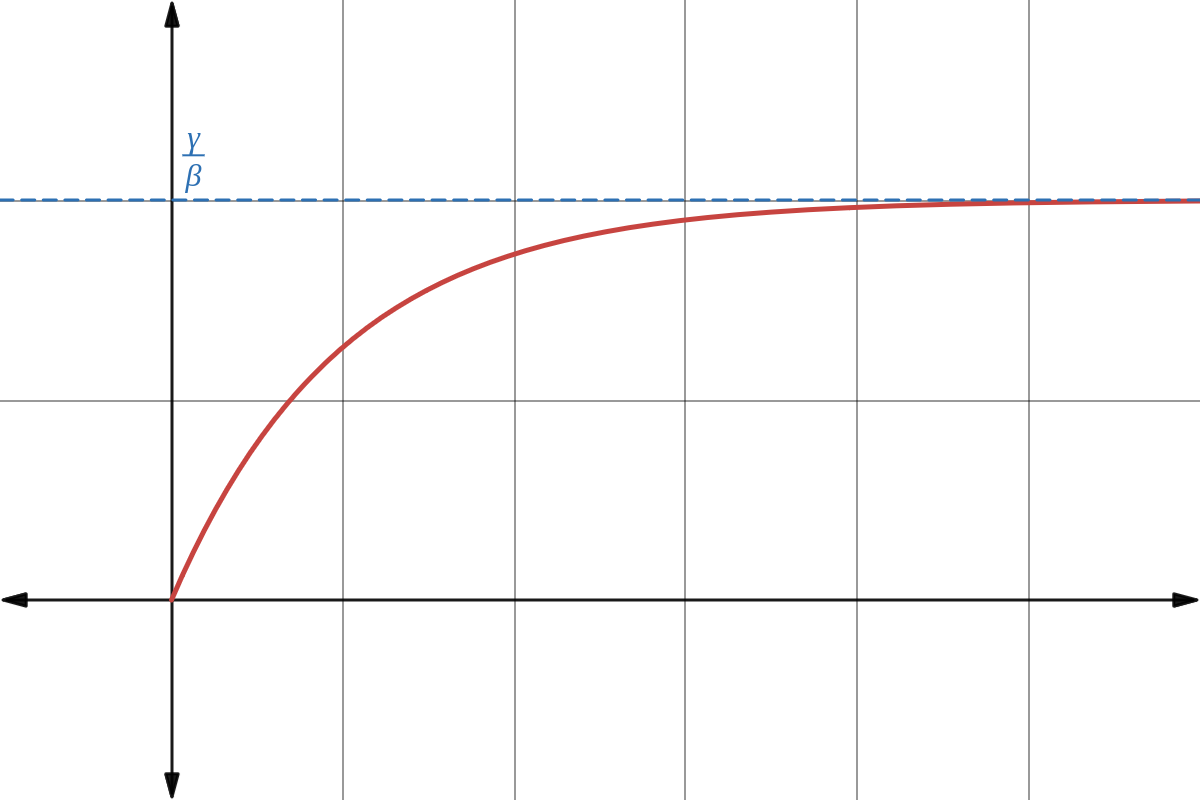
\includegraphics[scale=0.28]{../figures/crociera_first_order.png}
\end{center}
\end{minipage}

\subsubsection{Poli del sistema ed equazione caratteristica}
Si ha che i \textbf{poli} del sistema in forma a variabili di stato sono un \textit{sottoinsieme} degli \textbf{autovalori} della matrice $A$, in quanto li troviamo come radici dell'equazione:
$$
p_1(s) = \det(sI - A)
$$
al denominatore dell'inversa di $sI - a$, che corrisponde al polinomio caratteristico di $A$:
$$
p_2(s) = \det(A - \lambda I)
$$

Diciamo \textit{sottoinsieme} in quanto potrebbe esserci semplificazione fra numeratore e denominatore della funzione di trasferimento.
Quindi, non tutti gli autovalori della matrice $A$ diventeranno poli della funzione di trasferimento.
In particolare, dalla definizione di raggiungbilità ed osservabilità che avevamo dato, abbiamo che per ogni funzione di trasferimento $g_{ij}(s)$, i poli della funzione di trasferimento sono tutti e soli i poli (modi) raggiungibili dall'ingresso $u_j$ ed osservabili dall'uscita $y_i$.

Questo discorso tornerà utile quando discuteremo la differenza fra stabilità e \textit{BIBO} stabilità.

\subsection{Stabilità nel modello a funzione di trasferimento}
Abbiamo lavorato finora col modello a funzione di trasferimento, definita come:
$$
G(s) = \frac{\sum_{i = 0}^m b_i s^i}{\sum_{i = 0}^n a_i s^i} = \frac{ b_m (s - z_1) (s - z_2) ... (s - z_m) }{ a_n (s - p_1) (s - p_2) ... (s - p_n) }
$$
con $z_i$ gli $m$ \textit{zeri}, $p_i$ gli $n$ \textit{poli}, e $n > m$.

Di questa avevamo individuato le due forme:
\begin{itemize}
	\item \textbf{Forma di Evans:} evidenzia poli e zeri:
		$$
G(s) = \frac{\sum_{i = 0}^m b_i s^i}{\sum_{i = 0}^n a_i s^i} = \frac{ b_m (s - z_1) (s - z_2) ... (s - z_m) }{ a_n (s - p_1) (s - p_2) ... (s - p_n) }
		$$
	\item \textbf{Forma di Bode:} evidenzia le costanti tempo: 
		$$
G(s) = K \frac{ (\tau_a s + 1) (\tau_b s + 1) ... (\tau_i s + 1) }{ (\tau_1 s + 1) (\tau_2 s + 1) ... (\tau_n s + 1) }
		$$
\end{itemize}

Definiamo quindi formalmente \textbf{poli}:
\begin{definition}{Polo}
	Un polo $a_i$ di una funzione di trasferimento $G(s)$ è un valore di $s$ per cui $G(s)$ tende ad infinito:
	$$
	F(s) = \frac{g(s)}{\prod_{i = 1}^x (s - a_i)^n_i}
	$$
	con $n_i$ ordine del polo.
\end{definition}
e \textbf{zeri}:
\begin{definition}{Zeri}
	Uno zero $a_i$ di una funzione di trasferimento $G(s)$ è un valore di $s$ per cui $G(s)$ tende a zero: 
	$$
	F(s) = \frac{\prod_{i = 1}^x (s - a_i)^m_i}{g(s)}
	$$
	con $m_i$ ordine dello zero.
\end{definition}

Quello che ci interesserà nella valutazione della \textbf{stabilità} dei sistemi sarà la posizione dei poli nel piano complesso.
In particolare, come avevamo detto per i modi nel modello a variabili di stato, poli a componente \textit{reale negativa} danno \textbf{stabilità asintotica}, poli a componente \textit{reale nulla} danno \textbf{stabilità marginale}, e poli a componente \textit{reale positiva} dano \textbf{instabilità}.
Inoltre la componente \textit{complessa} dà informazioni sull'oscillazione del sistema, con \textbf{oscillazioni smorzate} a componente \textit{complessa e reale non nulle}, e \textbf{oscillazioni continue} a componente \textit{reale nulla}.

Gli zeri, invece, non hanno effetto sulla stabilità.
Gli zeri a parte reale positiva hanno invece l'effetto di \textit{invertire} la risposta al gradino, almeno sul breve termine.

\subsubsection{Stabilità e autovalori}
Avevamo che si poteva passare da modello a variabili di stato a funzione di trasferimento come:
$$
G(s) = \frac{Y(s)}{U(s)} = C(sI - A)^{-1} B + D = \frac{n(s)}{d(s)}
$$

Chiaramente, $n(s)$ e $d(s)$ saranno i polinomi di cui ci interessavamo per il calcolo di poli e zeri, di cui abbiamo detto ad interessarci per la stabilità erano i soli poli.
Ora, visto che abbiamo detto che c'è una qualche corrispondenza fra poli e autovalori, avremo che si può controllare la stabilità dai soli autovalori della matrice $A$.
Questo è infatti esattamente quello che avevamo fatto nel modello a variabili di stato.

\subsubsection{Stabilità BIBO}
Per parlare propriamente di stabilità, in relazione all'ingresso, nei modelli a funzione di trasferimento, introduciamo la nozione di sistema \textbf{BIBO} \textit{Bounded Input, Bounded Output}:
\begin{definition}{Sistema BIBO}
	Un sistema si dice stabile BIBO se ad ogni ingresso limitato corrisponde un'uscita limitata.
\end{definition}

Si ha che, per sistemi lineari, la stabilità BIBO si ha se e solo se i poli della funzione di trasferimento hanno tutti parte reale $< 0$.
Notiamo che la stabilità BIBO, al confronto della stabilità semplice che avevamo valutato finora, non dipende soltanto dallo stato interno del sistema, ma dalla \textbf{risposta forzata}.

\subsubsection{Poli dominanti}
In un sistema BIBO stabile, quindi, i modi sono tutti segnali esponenzialmente smorzati.
Al di là del transitorio iniziale, in questa situazione si avrà che il comportamento prevalente del sistema è quello dei modi più lenti, cioè quelli più vicini all'asse immaginario.

\subsubsection{Riassunto sulla stabilità}
Abbiamo quindi che \textbf{stabilità interna} (quella che avevamo visto nei modelli a variabili di stato) e \textbf{BIBO stabilità} di un sistema sono caratteristiche legate fra di loro ma separate:
\begin{table}[h!]
	\center \rowcolors{2}{white}{black!10}
	\begin{tabular} { c || p{5cm} | p{5cm} }
	& \bfseries Stabilità interna & \bfseries BIBO stabilità \\ 
	\hline 
		\bfseries Derivazione & Dagli autovalori (modi) della matrice $A$. & Dai poli della funzione di trasferimento, \\ 
		\bfseries Comportamento & Comportamento naturale, a partire dalle condizioni iniziali. & Sottoposto a un ingresso (risposta forzata) $u$ variabile $\neq 0$.
	\end{tabular}
\end{table}

La stabilità interna implica solitamente la stabilità BIBO, ma questo potrebbe non essere il caso se ci sono cancellazioni.
Possono esistere infatti esempi di sistemi BIBO stabili ma non internamente stabili, e viceversa.

Nel primo caso, il sistema potrebbe sembrare stabile "agli effetti esterni", ma determinate eccitazioni potrebbero portare a comportamenti instabili (oscillazioni incontrollate, ecc...), che solitamente raggiungono stati fisicamente 
impossibili all'interno del sistema stesso, e quindi fallimento.

Nel secondo, si potrebbero avere sistemi "di per sé" stabili, ma che rispondono in maniera negativa anche a piccolissime sollecitazioni esterne, rendendoli effettivamente instabili dal punto di vista della dinamica agli effetti esterni.

\subsection{Stabilità di sistemi in circuito chiuso}
Avevamo detto che i poli del sistema sono quelli che decidono la stabilità di un sistema.

\noindent
\begin{minipage}{\textwidth}
Preso ad esempio il sistema in ciclo chiuso:

\begin{center}
	\begin{tikzpicture}
		\draw (1,0) rectangle (3, 1);
		\node at (2, 0.5) {$G(s)$};
		
		\draw (-3,0) rectangle (-1, 1);
		\node at (-2, 0.5) {$C(s)$};

		\draw (-1.5, -0.5) rectangle (0.5, -1.5);
		\node at (-0.5, -1) {$H(s)$};

		\draw[-stealth] (-7, 0.5) -> (-5.1, 0.5);
		\draw[-stealth] (-5, 0.5) -> (-3, 0.5);
		\draw[-stealth] (-1, 0.5) -> (1, 0.5);
		\draw[-stealth] (3, 0.5) -> (3.9, 0.5);
		\draw[-stealth] (4, 0.5) -> (7, 0.5);
		
		\draw (5, 0.5) -> (5, -1);
		\draw[-stealth] (5, -1) -> (0.5, -1);
		\draw (-1.5, -1) -> (-5, -1);
		\draw[-stealth] (-5, -1) -> (-5, 0.5);

		\draw[-stealth] (4, 1.5) -> (4, 0.6);
		\node at (4, 1.75) {disturbo};

		\draw[fill=white] (-5, 0.5) circle (0.1);
		\draw[fill=white] (4, 0.5) circle (0.1);

		\node at (-6, 0.75) {$R(s)$};
		\node at (6, 0.75) {$Y(s)$};

		\node at (-4.75, 0.75) {$+$};
		\node at (-4.75, 0.25) {$-$};

		\node at (-3.8, 0.75) {\textit{errore}};
		\node at (0, 0.75) {\textit{controllo}};
		\node at (-3.5, -1.5) {\textit{feedback}};
	\end{tikzpicture}
\end{center}
\end{minipage}

\par\medskip

Dove le funzioni $C(s)$, $G(s)$ e $H(s)$ rappresentano rispettivamente il \textbf{controllore}, l'\textbf{impianto} e il \textbf{sensore}.
La funzione di trasferimento, trascurati i disturbi, avevamo detto era:
$$
\frac{Y(s)}{R(s)} = T(s) = \frac{C(s) G(s)}{1 + C(s)G(s)H(s)}
$$
da cui la stabilità del sistema è data dalla catena di retroazione completa (denominatore $d(s) = 1 + C(s)G(s)H(s))$, mentre la catena diretta $n(s) = C(s)G(s)$ dà solo gli zeri.

Del sistema in catena chiusa, quindi, valuteremo la stabilità controllando se i \textit{poli}  si trovano nella cosiddettà \textbf{regione di stabilità}, individuata come l'insieme di $z$ sul piano complesso a $\mathrm{Re}(z) < 0$.

Possiamo generalizzare il seguente discorso prendendo due funzioni di trasferimento, dette $G_{OL}$ (\textit{Open Loop}, in \textbf{anello aperto}), e $G_{CL}$ (\textit{Closed Loop}, in \textbf{anello chiuso}).
A questo punto potremo definire la funzione di trasferimento come:
$$
\frac{Y(s)}{R(s)} = T(s) = \frac{G_{OL}(s)}{1 + G_{CL}(s)}
$$
Notiamo che $G_{CL}$ è quanto si rileva dall'uscita attraverso il sensore, cioè:
$$
G_{CL}(s) = G_{OL}(s) H(s)
$$
e se $H(s) = 1$, la funzione di trasferimento sarà:
$$
\frac{Y(s)}{R(s)} = T(s) = \frac{G_{OL}(s)}{1 + G_{OL}(s)} \quad (H(s) = 1)
$$
Notiamo nuovamente che sarà solo il denominatore, in entrambi i casi, ad importarci per quanto riguarda la stabilità.

Facciamo alcuni esempi.

\subsubsection{Esempio: stabilità in catena chiusa}
Prendiamo il sistema con funzione di trasferimento in catena aperta:
$$
G_{OL} = \frac{10(0.5s + 1)}{s(2s + 1)}
$$
e trasferimento del sensore all'unità, e consideriamone la BIBO stabilità.
Vorremo prendere il solo denominatore:
$$
d(s) = 1 + G_{OL} = \frac{s(2s + 1) + 10(0.5s + 1)}{s(2s + 1)}
$$
di cui ci interessano solo gli zeri (cioè i poli di $T(s)$ funzione di trasferimento complessiva del sistema), quindi il numeratore::
$$
n'(s) = 2s^2 + s + 5s +10 = 2s^2 + 3s + 10
$$
di cui gli zeri:
$$
p_{1, 2} = \frac{-3}{4} \pm i \frac{\sqrt{79}}{4}
$$
con parte reale $< 0$, quindi il sistema è BIBO stabile.

\subsubsection{Esempio: stabilità in catena chiusa con parametro}
Prendiamo adesso un sistema con trasferimento in catena aperta determinato da un parametro:
$$
G_{OL} = s + 0.2 k - 2
$$
con transferimento del sensore sempre all'unità.
La domanda potrebbe essere per quali valori di $k$ il sistema è stabile.
Prendiamo allora il denominatore:
$$
d(s) = 1 + G_{OL} = s + 0.2 k - 1 \implies s = 1 - 0.2k
$$
di cui vediamo, se vogliamo poli in $s < 0$ e assumiamo $k \in \mathbb{R}$, dobbiamo imporre la condizione:
$$
k < 5
$$

\subsubsection{Esempio: stabilità in catena chiusa con parametro al second'ordine}
Facciamo un esempio analogo al precedente ma con una funzione di trasferimento del secondo grado:
$$
G_{OL} = \frac{k}{(2s + 1)(5s + 1)}
$$
con gli stessi assunti di prima sul sensore.
In questo caso il denominatore sarà:
$$
1 + G_{OL} = 1 + \frac{k}{(2s + 1)(5s + 1)} = \frac{10s^ + 7s  k + 1}{(2s + 1)(5s + 1)}
$$
da cui il numeratore:
$$
n'(s) = 10s^2 + 7s + k + 1
$$
per imporre $s < 0$, in questo caso, si dovrà dire:
$$
p_{1, 2} = \frac{-7 \pm \sqrt{49 - 40 (k + 1)}}{2(k + 1)}
$$
quindi parti reali:
$$
\mathrm{Re}(p_{1,2}) = -\frac{7}{2(k + 1)}
$$
e $k < -1$.

\subsection{Criterio di Routh}
Il \textbf{criterio di Routh} (\textit{criterio di Routh-Hurwitz}) è il primo metodo che vediamo per sistematizzare il procedimento di valutazione della stabilità.
Rappresenta un metodo \textit{puramente algebrico} che si applica a sistemi di controllo lineari tempo invarianti (\textit{LTI}).

Di base abbiamo che considereremo equazioni caratteristiche in forma polinomiale:
$$
p(s) = a_n s^n + a_{n - 1}s^{n - 1} + ... + a_1 s + a_0 = 0
$$
ciò che ci interessa è capire, guardando solo ai coefficienti $a_n, ..., a_0$, il segno delle componenti reali delle radici del polinomio, e in particolare sapere se queste sono tutte negative.
Il criterio di Routh ci permette di fare esattamente questo.

Vediamo innanzitutto le \textbf{condizioni di applicabilità}.
Abiamo la condizione necessaria ma non sufficiente per la stabilità, che tutti gli $n + 1$ coefficienti del polinomio devono avere lo stesso segno.
Questa è fra l'altro necessaria e sufficiente per $n \leq 2$.

Vorremo quindi calcolare la cosiddetta \textbf{tabella di Routh}.
Per un polinomio di grado $n$, questa avrà $n + 1$ righe.
Le prime due righe sono sempre costituite dai coefficienti del polinomio $p(s)$, distinto in una parte pari e una parte dispari.
Cioè assunto $n$ pari:
\[
	\begin{cases}
		p_1(s) = a_n s^N + a_{n - 2} s^{n - 2} + ... + a_0 \quad \hspace{0.85cm} \text{(pari)} \\
		p_2(s) = a_{n - 1} s^{n - 1} + a_{n - 3} s^{n - 3} + ... + a_1 s \quad \text{(dispari)}
	\end{cases}
\]

Potremo quindi dire:
\begin{table}[h!]
	\center 
	\begin{tabular} { c | c c c c }
		$n$ & $a_n$ & $a_{n - 2}$ & $a_{n - 4}$ & ... \\
		$n - 1$ & $a_{n - 1}$ & $a_{n - 3}$ & $a_{n - 5}$ & ... \\
		$n - 2$ & $b_1$ & $b_2$ & $b_3$ & ... \\
		$\vdots$ & ... & ... & ... \\
		1 & $y_1$ & $y_2$ \\
		0 & $z_1$
	\end{tabular}
\end{table}

Per i termini successivi si prende, ad esempio alla terza riga:
$$
b_1 = - \frac{ \det \begin{pmatrix}
	a_n & a_{n - 2} \\
	a_{n - 1} & a_{n - 3}
\end{pmatrix} }{a_{n - 1}}, \quad
b_2 = - \frac{ \det \begin{pmatrix}
	a_n & a_{n - 4} \\
	a_{n - 1} & a_{n - 5}
\end{pmatrix} }{a_{n - 1}}, \quad ...
$$
e cosi via per righe successive, cioè ogni volta si prende il minore ottenuto prendendo le due righe alla prima colonna  alla $i + 1$-esima dove $i$ è la colonna che consideriamo.
Vediamo che questo procedimento riduce automaticamente il numero di colonne di $1$ ogni $2$ righe (per gli elementi che rimangono \textit{a metà}, cioe non sono definiti sulla riga corrente, si prende 0).

Sulla tabella di Routh si possono dimostrare 2 teoremi, il primo riguardo alla condizione che cercavamo:
\begin{theorem}{Primo teorema di Routh}
	Condizione necessaria e sufficiente perchè tutte le radici dell'equazione caratteristica abbiano parte reale negativa è che tutti gli elementi della prima colonna della tabella di Routh siano positivi e non nulli.
\end{theorem}
e il secondo nel caso il primo fallisse:
\begin{theorem}{Secondo teorema di Routh}
	Se qualche elemento della prima colonna è negativo, il numero di radici con parte reale positiva è uguale al numero di cambi di segno dei coefficienti della prima colonna.
\end{theorem}

\end{document}
